% !TeX program = xelatex
\documentclass[12pt]{ctexbeamer}

\usetheme{metropolis}
\usepackage{appendixnumberbeamer}

\usepackage{booktabs}
\usepackage[scale=2]{ccicons}
\usepackage{tikz}
\usetikzlibrary{arrows,positioning,shapes.geometric,calc}

\usepackage{pgfplots}
\usepgfplotslibrary{dateplot}

\usepackage{xspace}
\newcommand{\themename}{\textbf{\textsf{STAEformer}}\xspace}

\setCJKmainfont[
    AutoFakeBold=true
]{FandolFang-Regular} % Beamer 默认使用 sf 字体族。

\setCJKsansfont[
    BoldFont=FandolSong-Bold,
    ItalicFont=FandolKai-Regular
]{FandolSong-Regular}

\setCJKmonofont[
    BoldFont=FandolHei-Bold
]{FandolHei-Regular}

\newCJKfontfamily\song[
    BoldFont=FandolSong-Bold
]{FandolSong-Regular}

\newCJKfontfamily\hei[
    BoldFont=FandolHei-Bold
]{FandolHei-Regular}

\newCJKfontfamily\kai[
    AutoFakeBold=true
]{FandolKai-Regular}

\newCJKfontfamily\fang[
    AutoFakeBold=true
]{FandolFang-Regular}


\title{STAEformer 模型架构分析}
\subtitle{时空自适应嵌入Transformer网络}
\date{\today}
\author{智能交通研究}
\institute{}

\begin{document}

\maketitle

\begin{frame}{目录}
	\setbeamertemplate{section in toc}[sections numbered]
	\tableofcontents[hideallsubsections]
\end{frame}

\section{模型概述}

\begin{frame}{STAEformer 整体架构}
	\begin{figure}
		\centering
		\begin{tikzpicture}[
				>=stealth,
				node distance=1.2cm and 1.5cm,
				block/.style={rectangle, draw, fill=blue!20, minimum width=2.2cm, minimum height=0.8cm, align=center, font=\small},
				arrow/.style={->, thick}
			]

			\node[block, fill=green!30] (input) {$X$ $(B, 12, 207, 3)$};
			\node[block, right=of input] (proj) {Input Projection};
			\node[block, fill=yellow!30, right=of proj] (embed) {时空自适应 嵌入融合};
			\node[block, fill=yellow!40, right=of embed] (temporal) {Temporal Attention};
			\node[block, fill=orange!40, right=of temporal] (spatial) {Spatial Attention};
			\node[block, fill=purple!30, right=of spatial] (ff) {Feed Forward};
			\node[block, fill=red!30, right=of ff] (output) {Mixed Projection};
			\node[block, fill=gray!30, right=of output] (result) {$\hat{Y}$ $(B, 12, 207, 1)$};

			\draw[arrow] (input) -> (proj);
			\draw[arrow] (proj) -> (embed);
			\draw[arrow] (embed) -> (temporal);
			\draw[arrow] (temporal) -> (spatial);
			\draw[arrow] (spatial) -> (ff);
			\draw[arrow] (ff) -> (output);
			\draw[arrow] (output) -> (result);

		\end{tikzpicture}
	\end{figure}
\end{frame}

\section{时空自适应嵌入}

\begin{frame}{自适应嵌入矩阵}
	\begin{figure}
		\centering
		\begin{tikzpicture}[
				>=stealth,
				node distance=0.6cm and 0.8cm,
				tensor/.style={rectangle, draw, fill=blue!20, minimum width=1.5cm, minimum height=1.2cm, align=center}
			]

			\node[tensor] (T) {$T_{in}=12$};
			\node[tensor, right=of T] (N) {$N=207$};
			\node[tensor, right=of N] (D) {$D_{adp}=80$};

			\node[below=0.8cm of T, font=\small] {时间步};
			\node[below=0.8cm of N, font=\small] {节点数};
			\node[below=0.8cm of D, font=\small] {嵌入维度};

			\node[right=2cm of D, tensor, fill=purple!30] (E) {$E_{adp}$};
			\node[right=0.4cm of E, font=\small] {$198\,720$ 参数};

		\end{tikzpicture}
	\end{figure}
\end{frame}

\begin{frame}{嵌入融合详情}
	\begin{table}
		\centering
		\begin{tabular}{lcc}
			\toprule
			嵌入类型        & 维度            & 说明                                                        \\
			\midrule
			Input Embed & 24维           & 线性投影 $W_{proj}: \mathbb{R}^3 \rightarrow \mathbb{R}^{24}$ \\
			ToD Embed   & 24维           & 时间 embedding, 288步/天                                      \\
			DoW Embed   & 24维           & 星期 embedding, 7天                                          \\
			Adaptive    & 80维           & 可学习参数 $E_{adp} \in \mathbb{R}^{12 \times 207 \times 80}$  \\
			\midrule
			\textbf{总计} & \textbf{152维} &                                                           \\
			\bottomrule
		\end{tabular}
	\end{table}
\end{frame}

\section{多头自注意力}

\begin{frame}{多头注意力机制}
	\begin{figure}
		\centering
		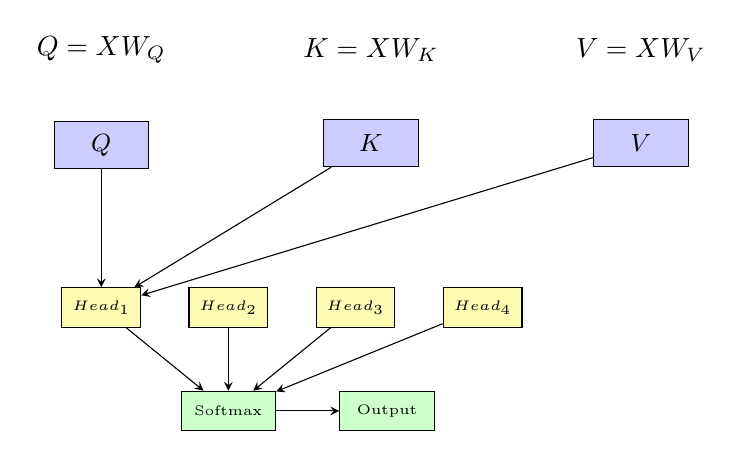
\begin{tikzpicture}[
				>=stealth,
				node distance=0.4cm and 0.8cm,
				qkv/.style={rectangle, draw, fill=blue!20, minimum width=1.2cm, minimum height=0.6cm, font=\small},
				head/.style={rectangle, draw, fill=yellow!30, minimum width=1cm, minimum height=0.5cm, font=\tiny},
				op/.style={rectangle, draw, fill=green!20, minimum width=1.2cm, minimum height=0.5cm, font=\tiny}
			]

			\node (Q) {$Q = XW_Q$};
			\node[right=1.5cm of Q] (K) {$K = XW_K$};
			\node[right=1.5cm of K] (V) {$V = XW_V$};

			\node[below=0.6cm of Q, qkv] (Qb) {$Q$};
			\node[below=0.6cm of K, qkv] (Kb) {$K$};
			\node[below=0.6cm of V, qkv] (Vb) {$V$};

			\node[below=1.5cm of Qb, head] (h1) {$Head_1$};
			\node[right=0.6cm of h1, head] (h2) {$Head_2$};
			\node[right=0.6cm of h2, head] (h3) {$Head_3$};
			\node[right=0.6cm of h3, head] (h4) {$Head_4$};

			\node[below=0.8cm of h2, op] (score) {Softmax};
			\node[right=0.8cm of score, op] (out) {Output};

			\draw[->] (Qb) -- (h1);
			\draw[->] (Kb) -- (h1);
			\draw[->] (Vb) -- (h1);

			\draw[->] (h1) -- (score);
			\draw[->] (h2) -- (score);
			\draw[->] (h3) -- (score);
			\draw[->] (h4) -- (score);

			\draw[->] (score) -- (out);

		\end{tikzpicture}
	\end{figure}
	\vspace{0.5cm}
	\centering
	公式:
	$$Attention(Q_i, K_i, V_i) = softmax\left(\frac{Q_i K_i^T}{\sqrt{d_k}}\right) V_i$$
\end{frame}

\section{时空交替Transformer层}

\begin{frame}{STAE Layer 结构}
	\begin{figure}
		\centering
		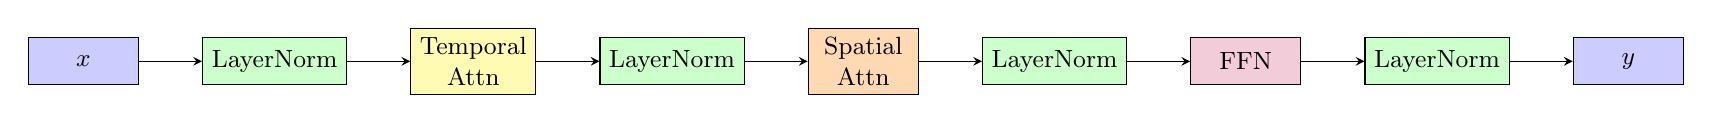
\begin{tikzpicture}[
				>=stealth,
				node distance=0.25cm and 0.8cm,
				layer/.style={rectangle, draw, fill=blue!20, minimum width=1.4cm, minimum height=0.6cm, font=\small, align=center}
			]

			\node[layer] (x) {$x$};
			\node[layer, fill=green!20, right=of x] (ln1) {LayerNorm};
			\node[layer, fill=yellow!30, right=of ln1] (ta) {Temporal\\Attn};
			\node[layer, fill=green!20, right=of ta] (ln2) {LayerNorm};
			\node[layer, fill=orange!30, right=of ln2] (sa) {Spatial\\Attn};
			\node[layer, fill=green!20, right=of sa] (ln3) {LayerNorm};
			\node[layer, fill=purple!20, right=of ln3] (ff) {FFN};
			\node[layer, fill=green!20, right=of ff] (ln4) {LayerNorm};
			\node[layer, right=of ln4] (y) {$y$};

			\draw[->] (x) -> (ln1);
			\draw[->] (ln1) -> (ta);
			\draw[->] (ta) -> (ln2);
			\draw[->] (ln2) -> (sa);
			\draw[->] (sa) -> (ln3);
			\draw[->] (ln3) -> (ff);
			\draw[->] (ff) -> (ln4);
			\draw[->] (ln4) -> (y);

		\end{tikzpicture}
	\end{figure}
	\vspace{0.3cm}
	\centering
	STAE Layer $\times$ 3
\end{frame}

\begin{frame}{Mixed Projection 输出}
	\begin{figure}
		\centering
		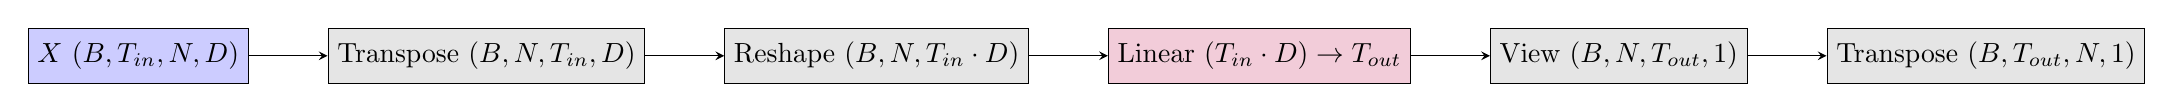
\begin{tikzpicture}[
				>=stealth,
				node distance=0.4cm and 1cm
			]

			\node[rectangle, draw, fill=blue!20, minimum width=1.8cm, minimum height=0.7cm] (x1) {$X$ $(B,T_{in},N,D)$};
			\node[rectangle, draw, fill=gray!20, minimum width=1.8cm, minimum height=0.7cm, right=of x1] (t) {Transpose $(B,N,T_{in},D)$};
			\node[rectangle, draw, fill=gray!20, minimum width=1.8cm, minimum height=0.7cm, right=of t] (r) {Reshape $(B,N,T_{in}\cdot D)$};
			\node[rectangle, draw, fill=purple!20, minimum width=1.8cm, minimum height=0.7cm, right=of r] (l) {Linear $(T_{in}\cdot D) \rightarrow T_{out}$};
			\node[rectangle, draw, fill=gray!20, minimum width=1.8cm, minimum height=0.7cm, right=of l] (v) {View $(B,N,T_{out},1)$};
			\node[rectangle, draw, fill=gray!20, minimum width=1.8cm, minimum height=0.7cm, right=of v] (t2) {Transpose $(B,T_{out},N,1)$};

			\draw[->] (x1) -> (t);
			\draw[->] (t) -> (r);
			\draw[->] (r) -> (l);
			\draw[->] (l) -> (v);
			\draw[->] (v) -> (t2);

		\end{tikzpicture}
	\end{figure}
\end{frame}

\section{模型配置}

\begin{frame}{模型参数配置}
	\begin{table}
		\centering
		\begin{tabular}{llr}
			\toprule
			参数                       & 默认值 & 说明            \\
			\midrule
			num\_nodes               & 207 & 节点数           \\
			in\_steps                & 12  & 输入时间步         \\
			out\_steps               & 12  & 输出时间步         \\
			steps\_per\_day          & 288 & 每日步数          \\
			input\_dim               & 3   & 输入维度          \\
			output\_dim              & 1   & 输出维度          \\
			input\_embedding\_dim    & 24  & 输入嵌入          \\
			tod\_embedding\_dim      & 24  & 时间嵌入          \\
			dow\_embedding\_dim      & 24  & 星期嵌入          \\
			adaptive\_embedding\_dim & 80  & 自适应嵌入         \\
			feed\_forward\_dim       & 256 & FFN维度         \\
			num\_heads               & 4   & 注意力头数         \\
			num\_layers              & 3   & Transformer层数 \\
			model\_dim               & 152 & 模型总维度         \\
			\bottomrule
		\end{tabular}
	\end{table}
\end{frame}

\section{总结}

\begin{frame}[standout]
	\centering
	\textbf{STAEformer} \\
	时空自适应嵌入 + Transformer架构 \\
	实现精准交通流预测
\end{frame}

\end{document}